\documentclass[aspectratio=169,xcolor=dvipsnames, t]{beamer}
\usepackage{fontspec} % Allows using custom font. MUST be before loading the theme!
\usetheme{SimplePlusAIC}
\usepackage{hyperref}
\usepackage{graphicx} % Allows including images
\usepackage{booktabs} % Allows the use of \toprule, \midrule and  \bottomrule in tables
\usepackage{svg} %allows using svg figures
\usepackage{tikz}
\usepackage{makecell}
\usepackage{wrapfig}
\usepackage[czech]{babel}
\usepackage{tabularx}
\newcommand{\R}{\mathbb{R}}
\newcommand{\N}{\mathbb{N}}


\title[]{Grafika, modely barev, barevná schémata} % The short title appears at the bottom of every slide, the full title is only on the title page
\subtitle{}

\author[Dusart]{Eric Dusart}
\institute[GEVO]{Gymnázium Evolution Jižní Město}
\date{\today}


\begin{document}

\maketitlepage
{
\setbeamertemplate{background}
{
    
\includegraphics[width=\paperwidth,height=\paperheight]{AICStyleData/logos/mene_polygonu_bg.png}
}
\begin{frame}[t]{Obsah}
    \tableofcontents
\end{frame}
}


\section{Grafika}
{
\setbeamertemplate{background}
{
    
\includegraphics[width=\paperwidth,height=\paperheight]{AICStyleData/logos/mene_polygonu_bg.png}
}
\begin{frame}{Vektorová grafika}
    \begin{itemize}
        \item .svg, .ps, .ai, .pdf
        \item Inkscape a další programy\ldots
        \item Bézierovy křivky
        \item Obrázek je složen z přesně definovaných bodů, přímek, křivek a mnohoúhelníků.
        \item Je možné neomezené bezztrátové zoomování.
        \item Je možné pracovat s každým objektem v obrázku odděleně.
        \item Výsledná paměťová náročnost obrázku je u jednolitých barevných obrázků menší, než při použití rastrového zápisu.
        \begin{itemize}
            \item Černé kolečko se uloží jako 3 informace: kruh, poloměr a výplň.
        \end{itemize}
        \item Většinou je těžší obrázek vytvořit.
        \item Větší projekty / obrázky jsou náročné na počítač (low pc skill issue).
        \item Nehodí se na obrázky, kde se hodně mění barvy a jsou složité, například fotografie.
    \end{itemize}
\end{frame}

\begin{frame}{Rastrová grafika}
    \begin{itemize}
        \item Pixely - body v nějakém gridu - matici.
        \item Body mají svoji polohu a svoji barvu v nějakém barevném modelu (třeba RGB).
        \item Kvalitu ovlivňuje rozlišení (počet pixelů) a barevná hloubka (počet bitů použitých k reprezentaci barvy pixelu)
    \end{itemize}
    \begin{figure}[H]
        \centering
        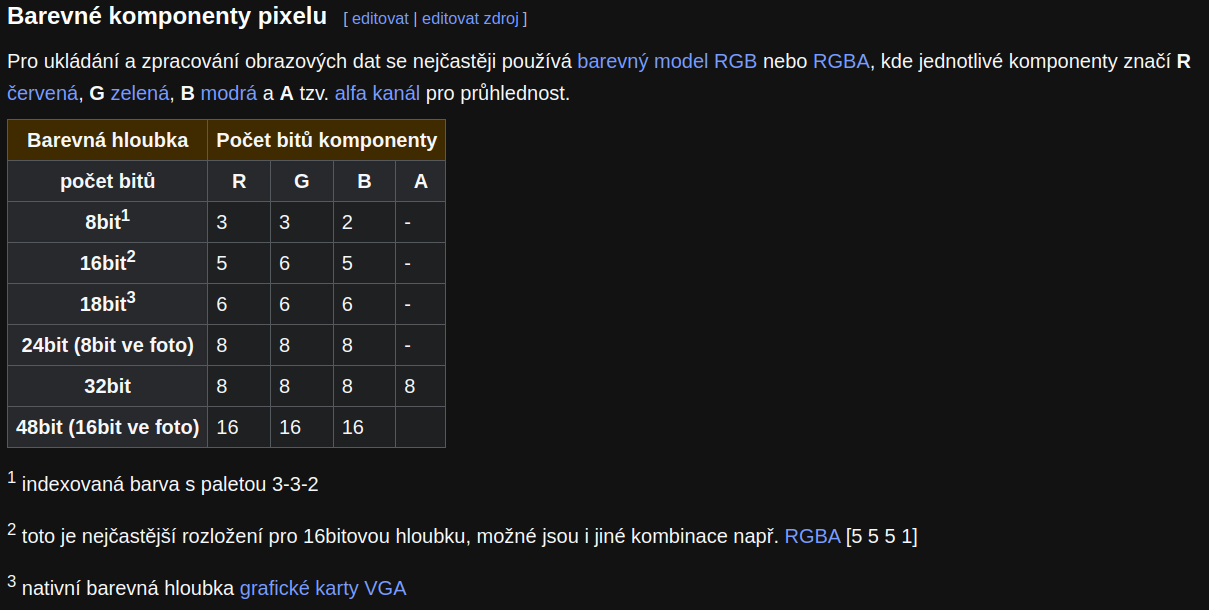
\includegraphics[width=0.5\textwidth]{a}
    \end{figure}
\end{frame}
\begin{frame}{Nějaké věci ve photoshopu}
    \begin{itemize}
        \item Praktická ukázka
        \item Vrstvy, masky, blending, adjustment layers
    \end{itemize}
\end{frame}

\section{Barevná schémata}
\begin{frame}{Barevná schémata}
    \begin{itemize}
        \item RGB, CMYK, YUV, HSL
        \item Jak ukládat barvy?
        \item Každý má své výhody a nevýhody.
        \item Ukaž colorpickery! (Připomeňte mi to, určitě na to zapomenu)
    \end{itemize}
\end{frame}
\begin{frame}{RGB}
\begin{itemize}
    \item Podle mezinárodní normy to je červená o vlnové délce 700 nm, zelená o vlnové délce 546,1 nm a modrá o vlnové délce 435,8 nm.
    \item (0, 0, 0) - černá, (255, 255, 255) - bílá
    \item Model založený na skládání barev.
    \item Nevhodný pro tisk, protože tisk využívá barvy odrážející světlo, nikoliv samotné světlo.
    \item Neodpovídá lidskému vnímání barev (např. změna jasu není lineární).
\end{itemize}
\end{frame}
\begin{frame}{CMYK}
    \begin{itemize}
        \item Cyan, Magenta, Yellow, Key/Black
        \item Používá se pro tisk.
        \item Založené na principu, že se světlo odráží od fyzického povrchu.
        \item Barvy vznikají odečítáním světla - čím více pigmentu, tím méně světla se odráží.
        \item Reálná černá, když vytiskneme černou v RGB (0, 0, 0), tak na papíře bude vypadat leehce \uv{šedě}, 
    \end{itemize}
\end{frame}

\begin{frame}{HSL}
    \begin{itemize}
        \item Percepční model - snaží se popsat barvy tak, jak je vnímá člověk.
        \item Hue (Odstín): pozice barvy na kruhu (0-360°, např. 0 = červená, 120 = zelená, 240 = modrá).
        \item Saturation (Sytost): čistota barvy (0 \% = šedá, 100 \% = plně sytá).
        \item Lightness (Světlost): jak moc světlá nebo tmavá je barva (0 \% = černá, 100 \% = bílá).
        \item Používá se v grafických editorech, web designu, atd\ldots
        \item Poměrně intuitivní pro člověka.
        \item Vhodný pro generování palet, gradientů, pastelových odstínů.
        \item Umožňuje snadno upravovat světelnost nebo sytost bez změny základního odstínu.
        \item Není optimalizován pro kompresi nebo věrné zobrazení barev.
    \end{itemize}
\end{frame}

\begin{frame}{YUV}
    \begin{itemize}
        \item Jasová složka Y a dvě barevné složky U, V.
        \item U a V jsou rozdíly barev oproti šedé.
        \item Používá se kvůli možnosti komprese bez výrazného snížení kvality.
        \item Umožňuje oddělit barevnou složku od světlosti (např. noční vidění může využívat pouze složku Y).
    \end{itemize}
\end{frame}

\begin{frame}{Srovnání barevných modelů}
    \centering
    \footnotesize % nebo \scriptsize pro úsporu místa
    % \renewcommand{\arraystretch}{1.3} % Více místa mezi řádky
    \begin{tabularx}{\textwidth}{l l l l X X}
        \toprule
        \textbf{Model} & \textbf{Typ} & \textbf{Založen na} & \textbf{Použití} & \textbf{Výhody} & \textbf{Nevýhody} \\
        \midrule
        RGB  & Aditivní   & Světlo         & Displeje, web      & Široký gamut, intuitivní pro zařízení & Nevhodný pro tisk, nelineární vnímání \\
        CMYK & Subtraktivní & Pigmenty     & Tisk               & Ideální pro tisk, ostrý text          & Malý gamut, rozdíly v tisku \\
        YUV  & Percepční  & Jas + barva    & Video, komprese    & Účinná komprese, šetří místo          & Neintuitivní, nutná konverze \\
        HSL  & Percepční  & Lidské vnímání & Design, UI         & Intuitivní úpravy, krásné palety      & Nepřesný pro výpočty, míchání \\
        \bottomrule
    \end{tabularx}
    
    * Gamut popisuje, jaké barvy je dané zařízení schopné zobrazit, případně zaznamenat.
\end{frame}
}

\finalpagetext{Děkuji za pozornost}
%----------------------------------------------------------------------------------------
\makefinalpage
%----------------------------------------------------------------------------------------
\end{document}
